\section{Evaluation}


\begin{figure*}[!htb]
	% \captionsetup[subfigure]{font=small,labelfont=small}
	% \begin{subfigure}[t]{0.2\textwidth}
	% 	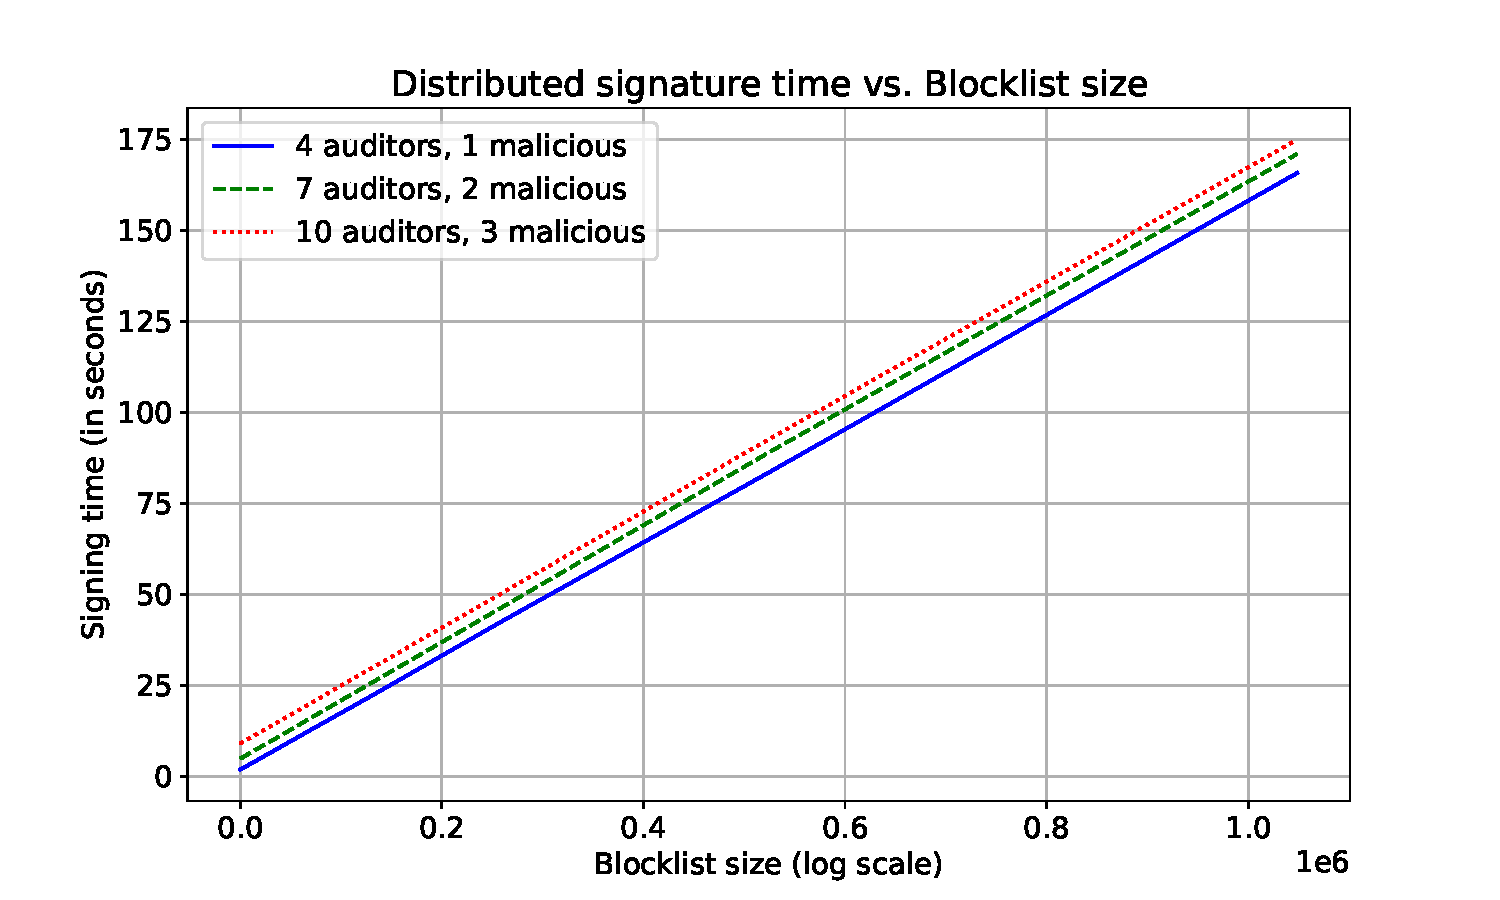
\includegraphics[scale=0.2]{plots/figs/server_sigtime.pdf}
	% 	\caption{\centering \footnotesize CPU time for signing blocklist (in seconds) }
	% 	\label{fig:dis_sign}
	% \end{subfigure}
	% \hfill
	\begin{subfigure}[t]{0.3\textwidth}
		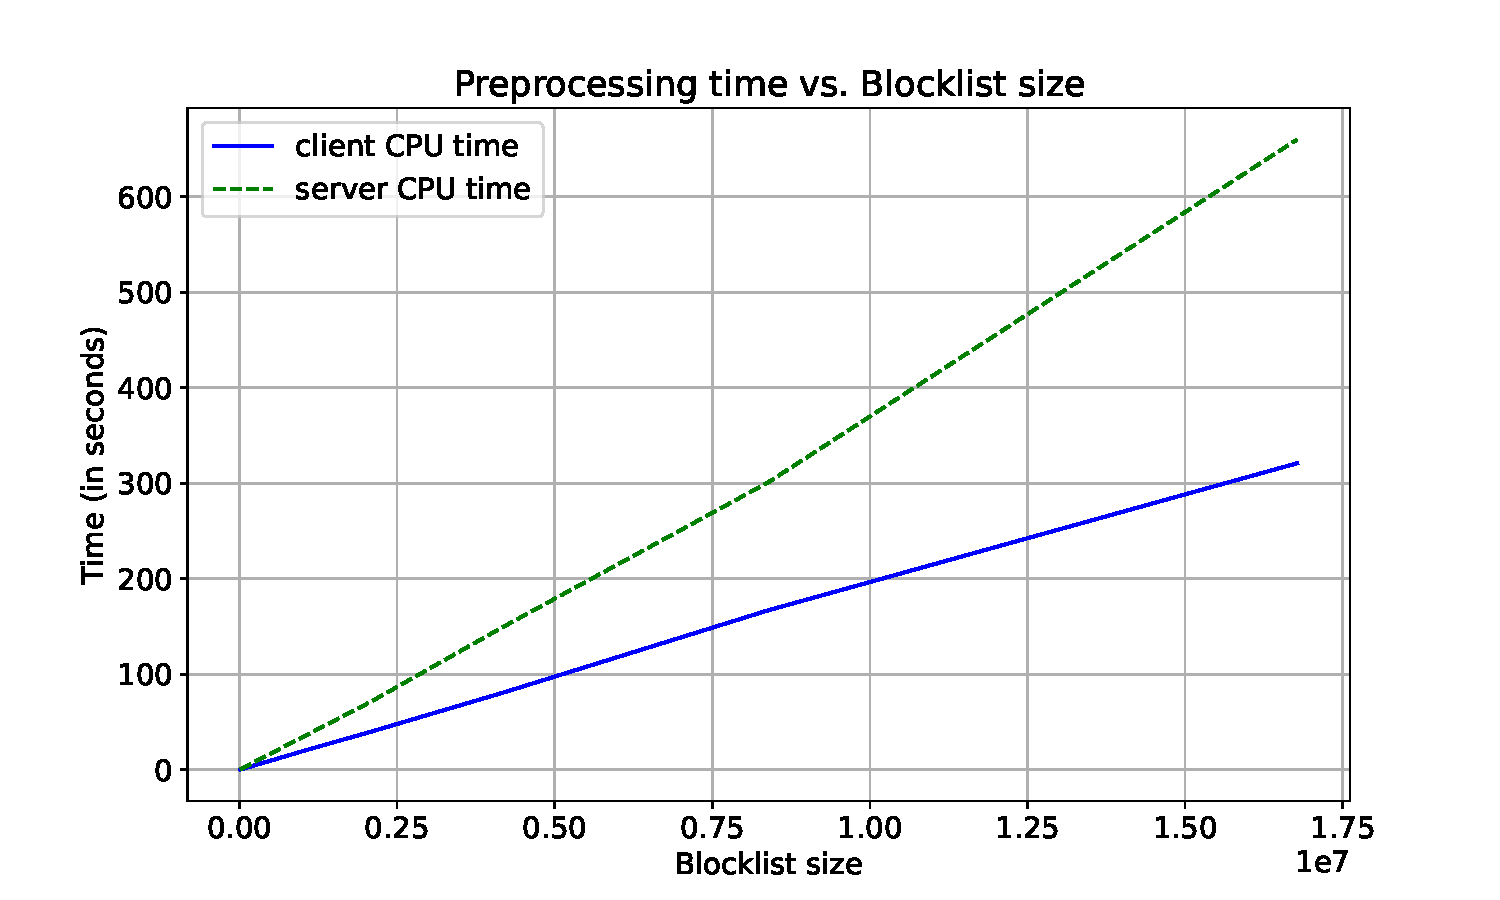
\includegraphics[scale=0.25]{plots/figs/client_preprocess_time_blocklistsize.pdf}
		\caption{\centering \footnotesize CPU time for preprocessing in \protocolEM (in seconds)} 
		\label{fig:cpu-preprocess}
	\end{subfigure}
	\hfill
	\begin{subfigure}[t]{0.3\textwidth}
		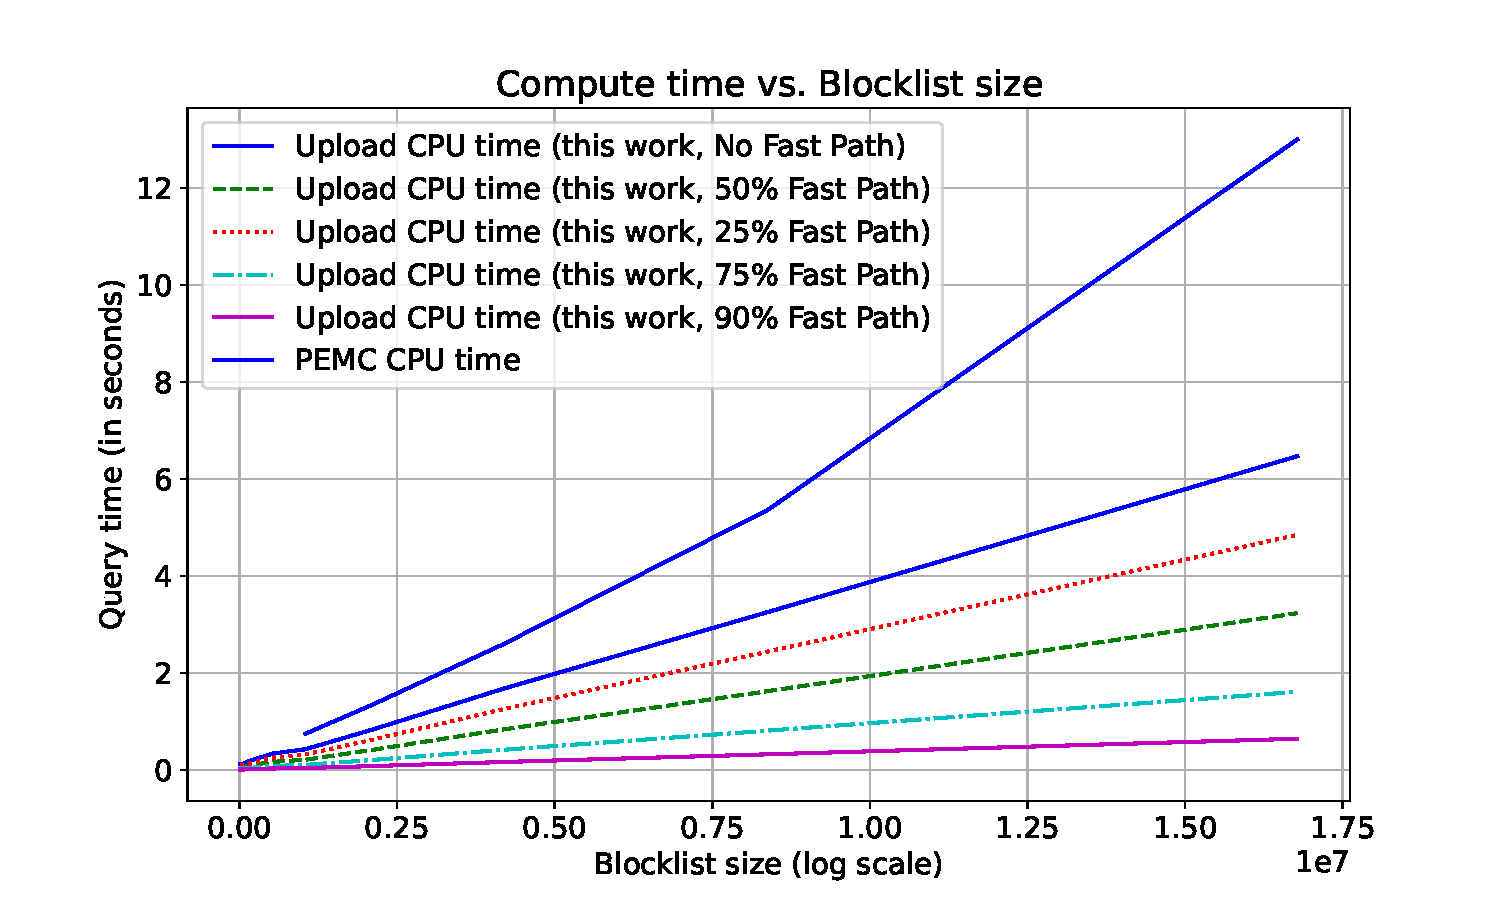
\includegraphics[scale=0.25]{plots/figs/server_sigtime_blocklistsize_pre.pdf}
		\caption{\centering \footnotesize Total upload time for \protocolEM (in seconds) }
		\label{fig:cpu-pre}
	\end{subfigure}
	\hfill
	\begin{subfigure}[t]{0.3\textwidth}
		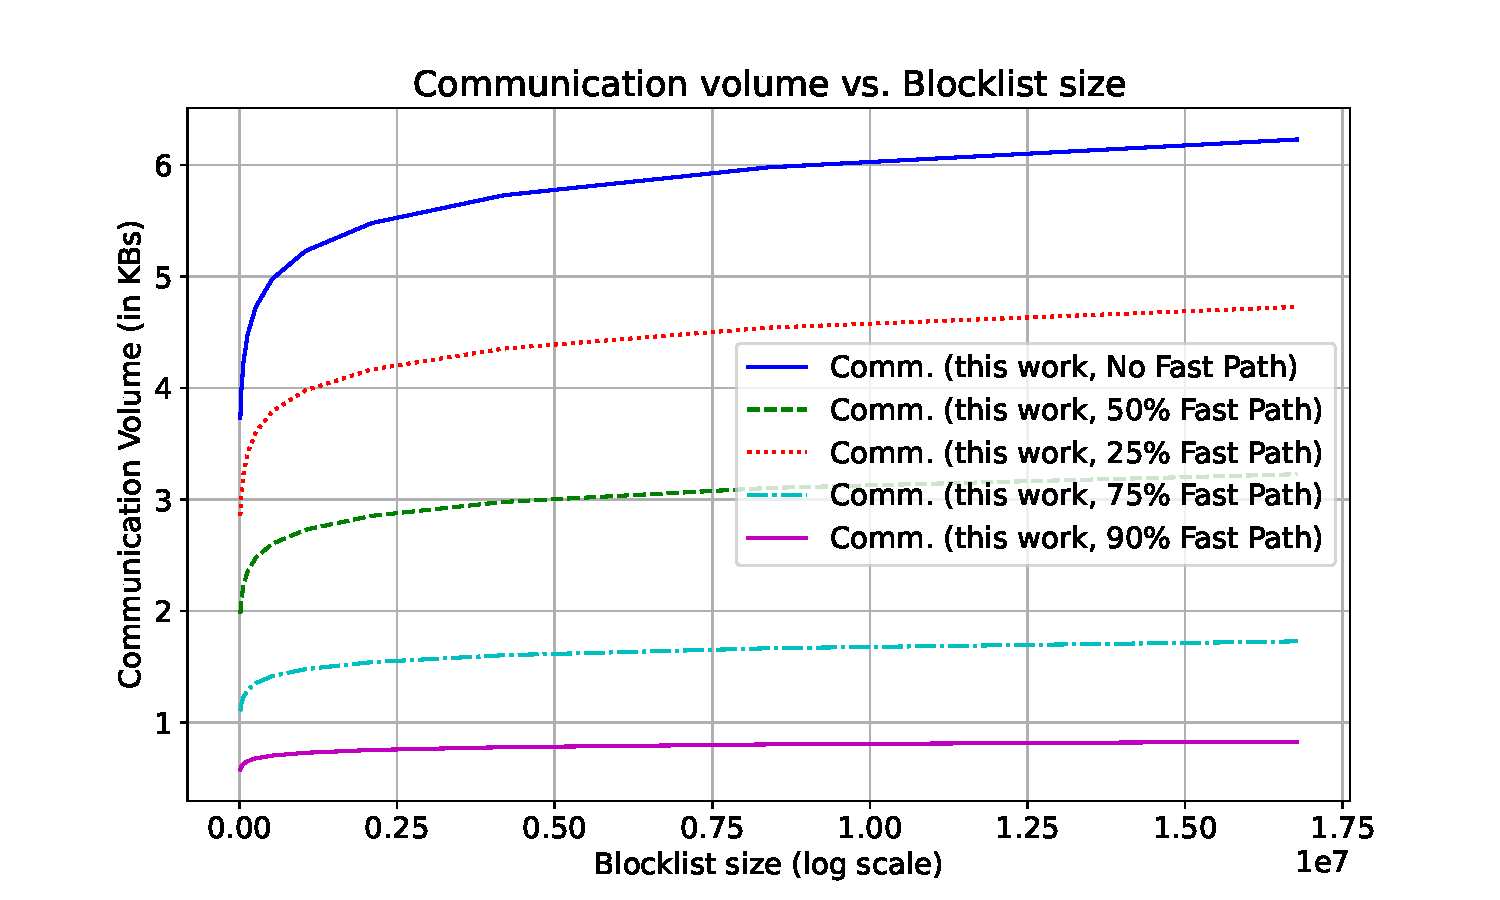
\includegraphics[scale=0.25]{plots/figs/server_comm_blocklistsize_pre.pdf}
		\caption{\centering \footnotesize Communication volume for \protocolEM (in KBs)}
		\label{fig:exact_comm}
	\end{subfigure}
%	\caption{\small Costs for content moderation with exact matching}
%	\label{fig:exact-match}
% \captionsetup[subfigure]{font=small,labelfont=small}
% 	\begin{subfigure}[t]{0.33\textwidth}
% 		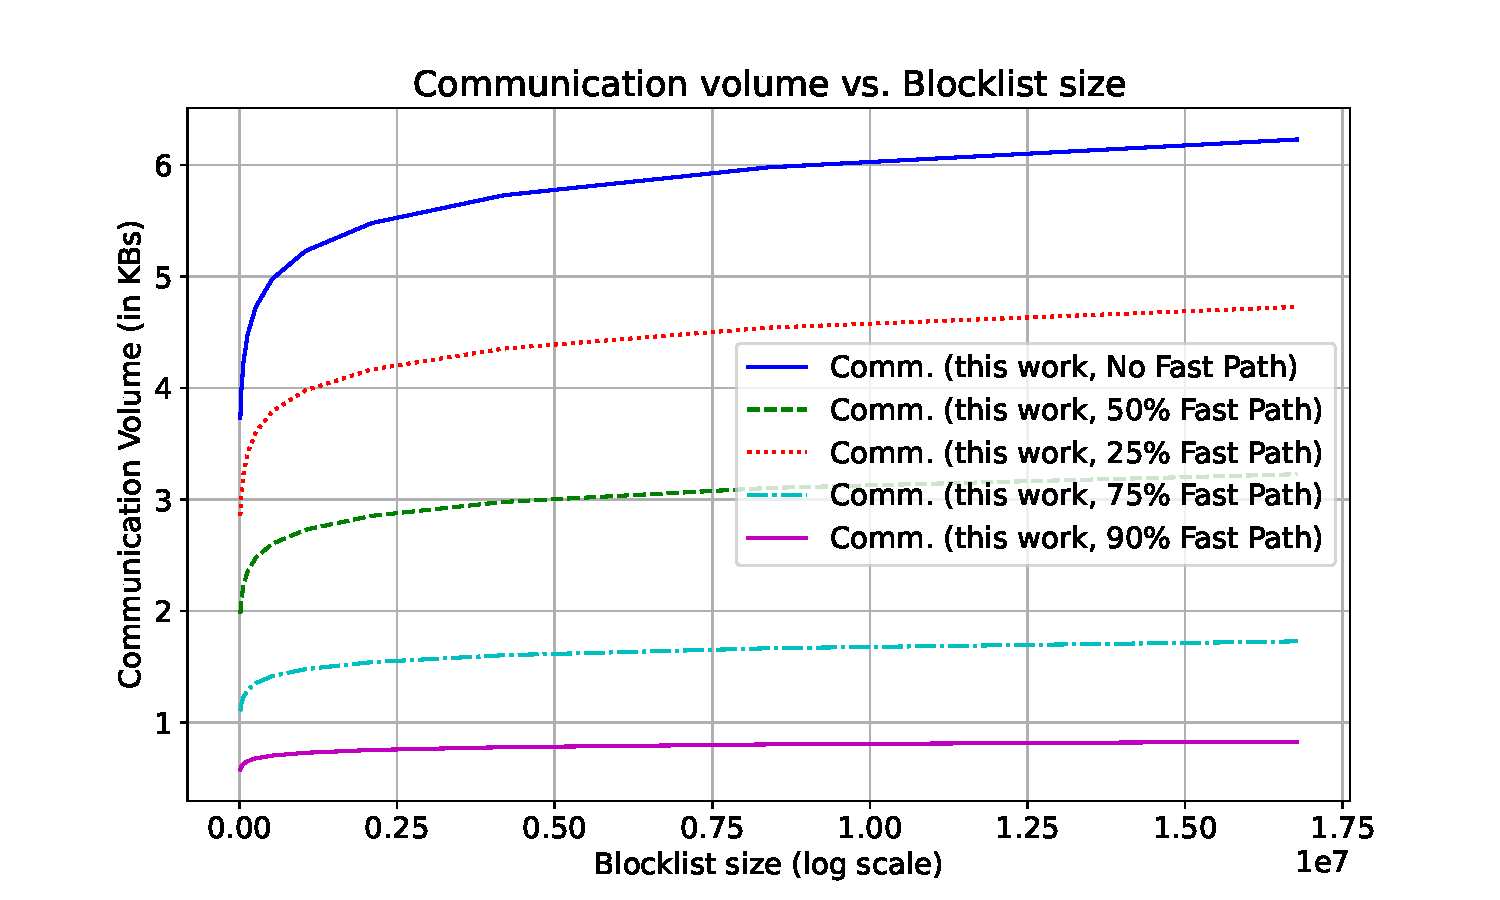
\includegraphics[scale=0.25]{plots/figs/server_comm_blocklistsize_pre.pdf}
% 		\caption{\centering \footnotesize Communication volume for \protocolEM (in KB)}
% 		\label{fig:exact_comm}
% 	\end{subfigure}
% 	\begin{subfigure}[t]{0.33\textwidth}
% 		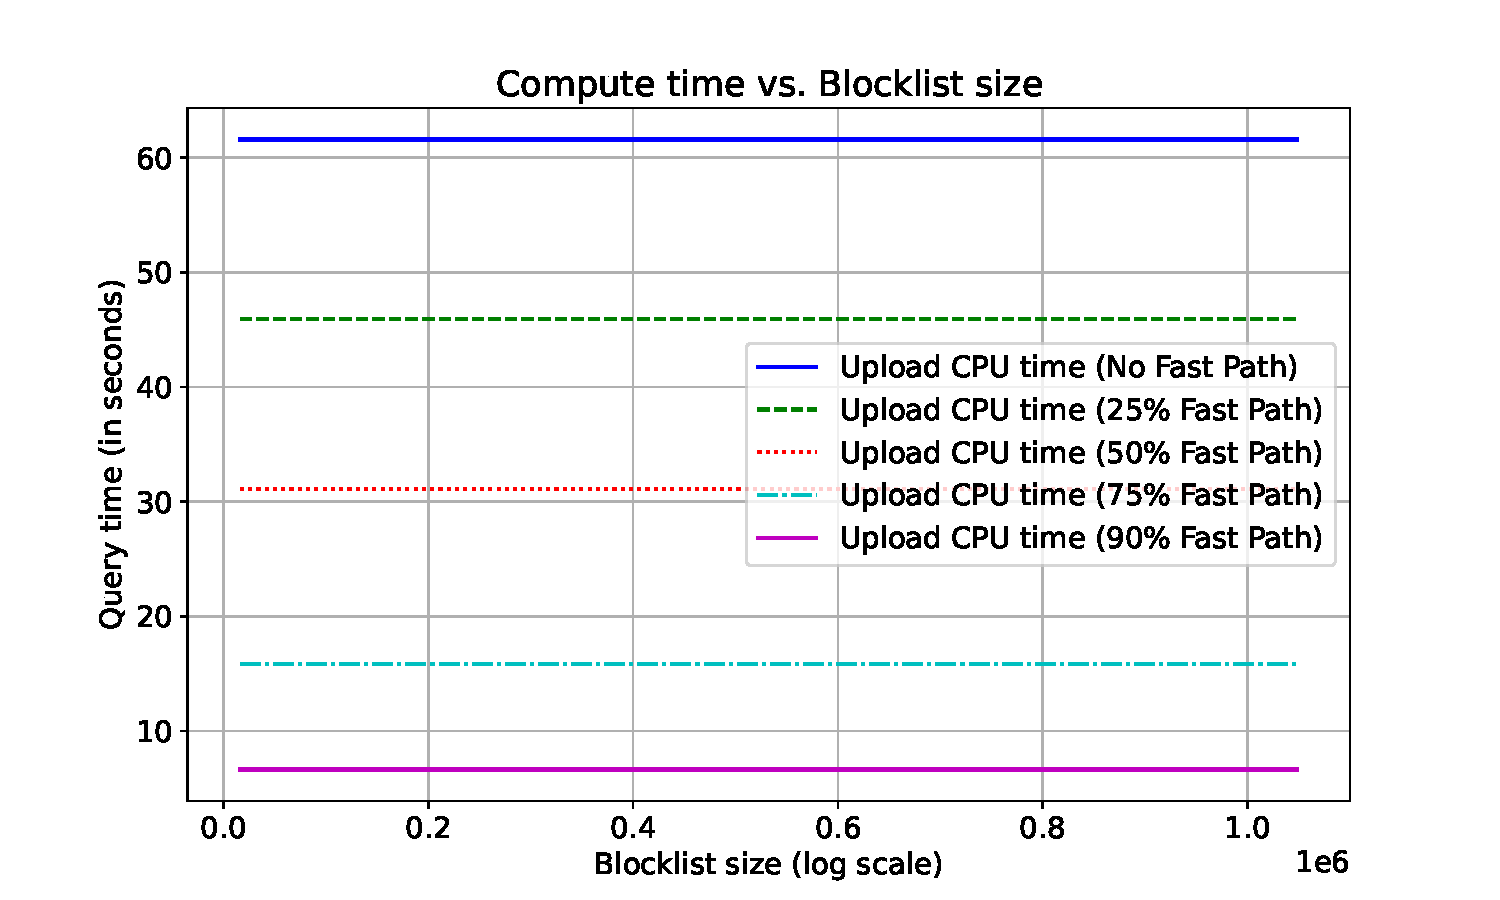
\includegraphics[scale=0.25]{plots/figs/server_sigtime_blocklistsize_pre_approx.pdf}
% 		\caption{\centering \footnotesize Total upload time for \protocolFM (in seconds)}
% 		\label{fig:cpu-pre-approx}
% 	\end{subfigure}
% 	\hfill
% 	\begin{subfigure}[t]{0.33\textwidth}
% 		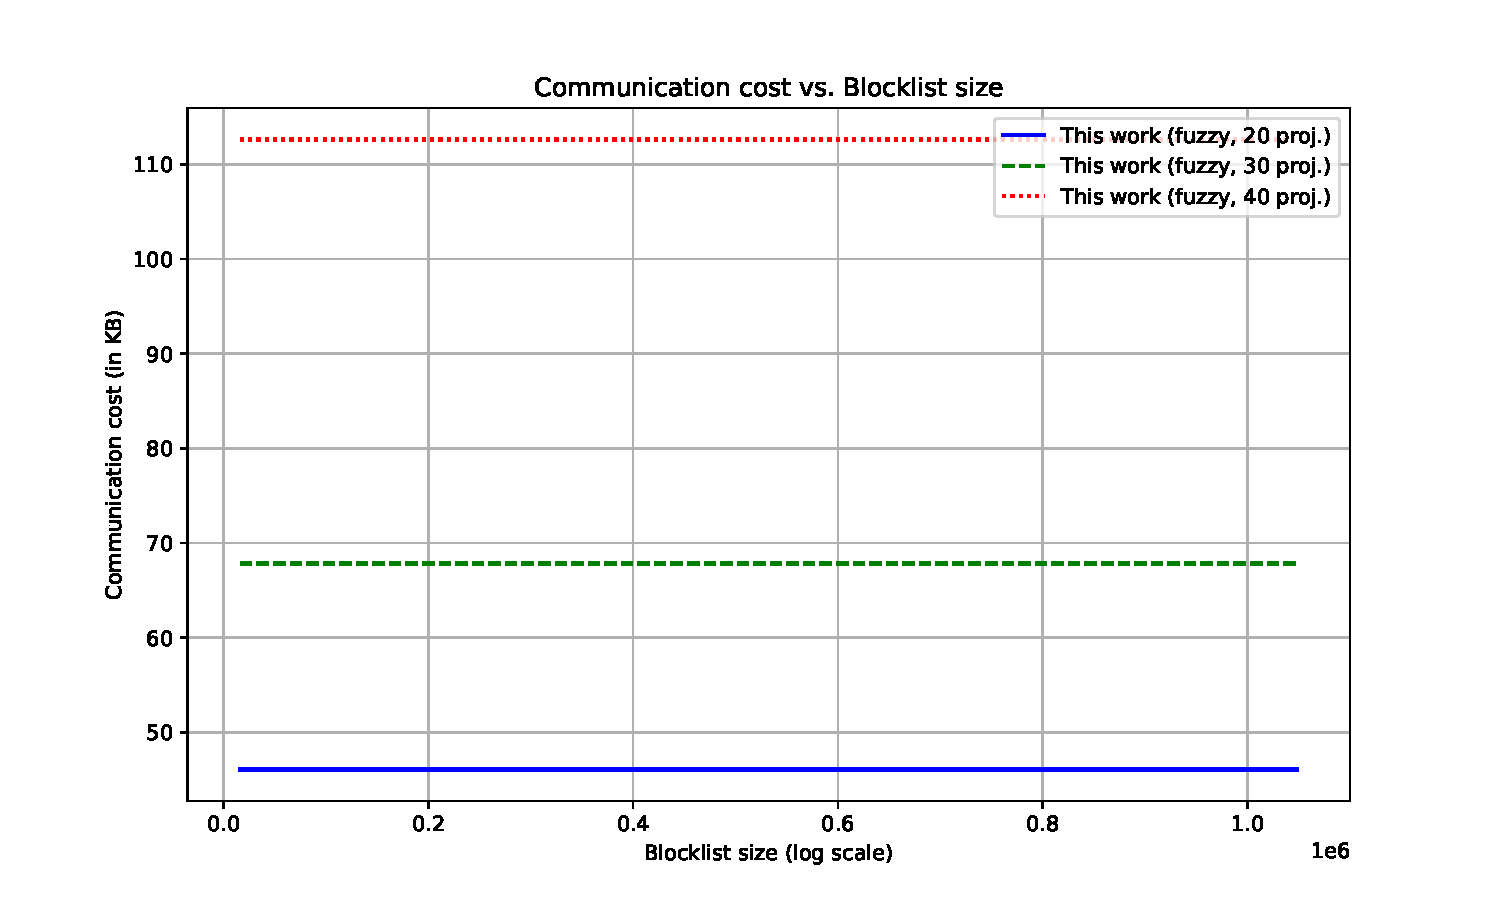
\includegraphics[scale=0.25]{plots/figs/client_comm_blocklistsize.pdf}
% 		\caption{\centering \footnotesize Communication volume for \protocolFM (in KB)} 
% 		\label{fig:storage}
% 	\end{subfigure}
% \vspace{-2pt}
% 	\caption{\small Costs for content moderation with exact and fuzzy matching}
% 	\label{fig:fuzzy-match}  
\end{figure*}








\begin{table}[t]
% \fontsize{5.6}{5.6} \selectfont
\footnotesize
% \tiny
\setlength{\tabcolsep}{2pt}
\begin{tabular}{| c | c | c | c | c |}
\noalign{\global\arrayrulewidth1pt}\hline\noalign{\global\arrayrulewidth0.4pt}
\multirow{2}{*}{DB size} & \multicolumn{2}{c|}{Our protocol \protocolFM} & \multicolumn{2}{c|}{PAMC~\cite[Table~8]{kulshrestha2021identifying}}\\  
\cline{2-5}
& Time (in sec.) & Comm. (in KB) & Time (in sec.) & Comm. (in KB)\\
\cline{1-5}
1048576 & 0.59 & 20  & 27.5 & 508\\
\cline{1-5}
2097152 & 0.59  & 20 & 27.5 & 586 \\
\cline{1-5}
4194304 & 0.59  & 20  & 27.7 & 742 \\
\cline{1-5}
8388608 & 0.59  & 20  & 28.3 & 1053.9 \\
\cline{1-5}
\end{tabular}
%\vspace{0.2em}
\caption{\small Comparison of \protocolFM against PAMC~\cite{kulshrestha2021identifying}\label{tab:comp}. }
\end{table}

All our protocols have been implemented and benchmarked\footnote{https://anonymous.4open.science/r/content-mod-code-2125/}. 
We implemented the protocols in C++ and Python. Group arithmetic was implemented using the NTL library\footnote{\url{https://libntl.org}}. The gRPC library\footnote{\url{https://grpc.io}} was used for implementing communication between the client and the server. For the OPRF and the partially homomorphic encryption scheme, we used the \emph{oblivious} library\footnote{\url{https://pypi.org/project/oblivious/}}, and the \emph{lightPHE} library~\cite{serengil2024lightphe} respectively. We used the exponential Elgamal encryption scheme for the additively-homomorphic encryption over the ED25519 elliptic curve. All parameters were configured to provide 112 bits of security. 
Benchmarks were performed with a single server running on an Amazon t2.2xlarge instance with 8vCPUs and 32GB of memory. Our implementations are single-threaded. Clients were run on a t2.large instance with 2vCPUs and 8GB of memory. 	


%\begin{figure}
%\begin{subfigure}[t]{0.25\textwidth}
%		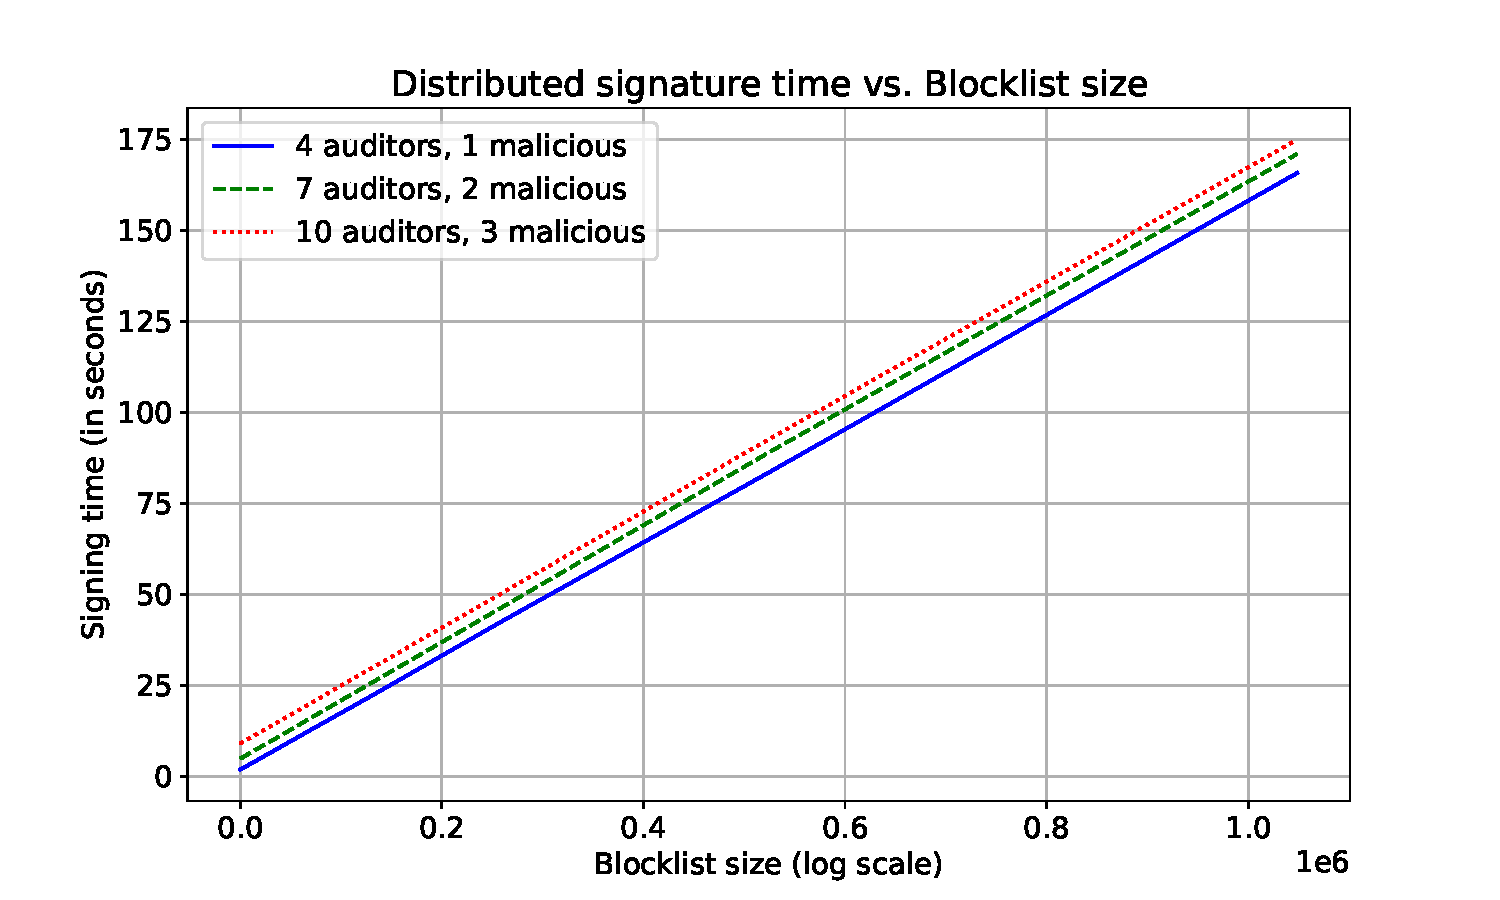
\includegraphics[scale=0.17]{plots/figs/server_sigtime.pdf}
%		\caption{\centering \footnotesize CPU time for signing blocklist}
%		\label{fig:sign}
%	\end{subfigure}
%	\begin{subfigure}[t]{0.18\textwidth}
%		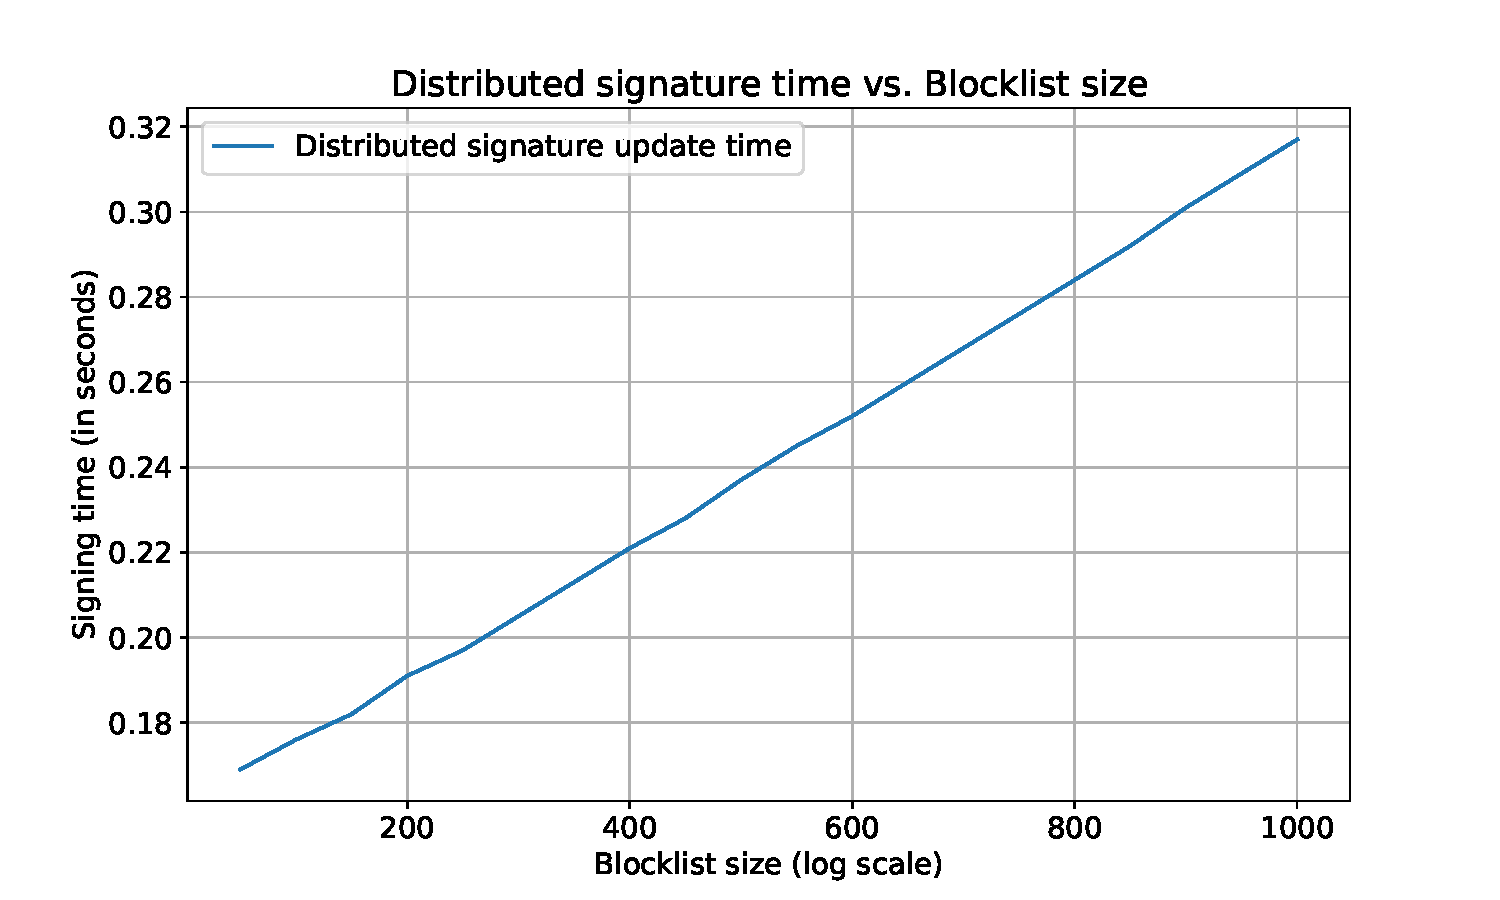
\includegraphics[scale=0.17]{plots/figs/server_sigtime_update.pdf}
%		\caption{\centering \footnotesize CPU time for updating signature} 
%		\label{fig:update}
%	\end{subfigure}
%\caption{CPU time for distributed signature and updates\label{fig:sig_time}}
%\end{figure}




\subsection{Exact Matching}
%
We conducted experiments for $\protocolEM$ using blocklists containing random SHA256 hashes. All tests were run 10 times and results were averaged across all runs. We compared our protocol with the PEMC protocol~\cite{kulshrestha2021identifying}\footnote{Their implementation is not publicly available but the paper reports benchmarks on a 6-core system with 32GB memory. For a fair comparison, we benchmarked our protocols on a similarly-provisioned system.}. \emph{We stress that our protocol works against a malicious server in contrast to the semi-honest server in case of PEMC}. 

%The Apple PSI system~\cite{bhowmick2021apple} also provide a mechanism for exact matching that tolerates a malicious server, but we did not find an implementation of this work, and the paper does not report benchmarks. Nonetheless, our solution has the same asymptotic costs as the Apple PSI system, and we improve on client storage costs and eliminate false negatives (see \secref{sec:related}). 


%
%
%For a blocklist with a million elements, the PEMC protocol requires 750 milliseconds of server + client compute time. In contrast, the server compute time in \protocolEM is 430 milliseconds when a fine grained check is performed against the \contentToken. The communication cost of our protocol is almost 3 orders of magnitude less than PEMC (718B vs. 400KB). This is because PEMC leverages a single-server PIR protocol over the entire blocklist, resulting in $\bigO(\sqrt{\blocklistSize})$ communication overhead per upload. 



\myparagraph{Publishing the blocklist}
%
\figref{fig:dis_sign} in the Appendix shows the compute costs for publishing the blocklist. We set the number of partitions $\numBlocklistParts$ such that each partition has at most 64 items. This  was fixed based on the time to perform a fine-grained match, if required. Signing a blocklist with a million items takes roughly 170 seconds with up to 10 auditors

%When a signature has to be updated, e.g., when new items are added to the blocklist, we can leverage the homomorphic properties of the signature scheme. Updating a signature with 1000 new items takes less than 0.5 seconds.

\myparagraph{Preprocessing}
%
\figref{fig:cpu-preprocess} shows the compute time required for preprocessing the blocklist. In our implementation, the OPRF of choice is the 2HashDH over curve25519\footnote{https://www.ietf.org/archive/id/draft-irtf-cfrg-ristretto255-00.html}. The number of bins in our implementation was fixed to $\blocklistSize/\log \blocklistSize$. For a million blocklisted items, preprocessing takes roughly 21 seconds for the client and 36 seconds for the server. 

\myparagraph{Uploads}
%
We benchmarked the upload time in \protocolEM by varying the fraction of queries that require a fast path verification (\figref{fig:cpu-pre}). The reported times are averaged over 1000 queries. In the most conservative case, where every upload results in a fine-grained check, the protocol requires roughly 430 milliseconds for a blocklist with a million items. In contrast, the PEMC protocol requires 750 milliseconds to perform the check. Moreover, when the fraction of queries served through a fast path verification increases, the compute times reduce proportionally. This feature is absent from the PEMC protocol, which runs a full check for every uploaded file. In fact, if we make a reasonable assumption that for a server detecting CSAM, a large fraction (90\%) of the content will not be blocklisted, \protocolEM achieves verification times of 43 ms per upload on average, a \textbf{12$\times$ compute cost improvement over PEMC}. 

\figref{fig:exact_comm} shows the communication costs of \protocolEM. Recall that the communication involves a Bloom filter for a specific bin, which in our cases has $\log \blocklistSize$ items, and $\log \blocklistSize$ signatures when a fine grained check is required. Even in the most conservative case when none of the uploads are served by a fast path, the communication required in \protocolEM for a 1 million-item blocklist is roughly 6KB. In comparison, PEMC requires 394KB since it performs a PIR over the blocklist. Thus, \protocolEM has \textbf{50$\times$ lower communication volume than PEMC}. 



\subsection{Fuzzy Matching}
%
We conducted experiments for our fuzzy matching protocol \protocolFM using a blocklist with random 256 bit vectors that simulate perceptual hashes. We instantiated the projection functions with the construction of \citet{chongchitmate2024approximate}.  We set the number of projections to 20 which gives a false positive rate $\badFP \le 0.02$ and $\badFN \le 0.07$. 

\myparagraph{Uploads}
%
We compared against the private approximate matching (PAMC) protocol~\cite{kulshrestha2021identifying} that only tolerates a semi-honest server and has a higher false negative rate of roughly $17\%$. \tblref{tab:comp} presents the results. We observe that  our protocol is faster (\textbf{by a factor of 5$\times$}) and requires less communication (\textbf{by at least a factor of 25$\times$}). The protocol of \citet{kulshrestha2021identifying} does not have any false positives because it computes the actual distance between the client's input and the blocklisted items, but this comes at the cost latencies that are unacceptable for a file store. In contrast, as discussed before, we tolerate a small amount of false positives (without leaking any infomration to the server) to have better performance while tolerating a malicious server. 

\myparagraph{Storage costs}
%
Both of our content moderation schemes require some client-side storage. For \protocolEM, a millions-sized blocklist requires roughly 4MB of storage for storing the the Bloom filter based ACB \bfBlklistToken,  for an overall false positive rate of $0.001$ in the fast path. The signature based ACB \sigBlklistToken also requires in total 4MB. Thus, the total storage cost is reasonable and less than 10MB. The CHT-based ACB \chtBlklistToken for the fuzzy match requires roughly 2.5GB for a million-sized blocklist with 20 projections. This is less than $5\%$ of the capacity of most commercially available smartphones with $\ge 64$GB of storage. 

% \figref{fig:cpu-pre-approx} demonstrates the compute costs of \protocolFM. In the conservative case where all uploads required a fine-grained check, \protocolFM requires around 61 seconds per upload. \emph{We recall that the cost of the protocol is independent of the blocklist size, and scales only in the number of projections and size of the vectors}.  Increasing the fraction of uploads served by fast path checks, proportionally reduces the compute costs. When $90\%$ of the uploads are served by the fast path (when blocklisted content is infrequently uploaded), the protocol requires less than 7 seconds per check on average. 


%\myparagraph{Costs without preprocessing}
%
%\figref{fig:cpu-nopre} presents the compute costs of the \protocolEM protocol described in \figref{fig:exact_match}. The client compute time is minimal requiring roughly 7ms to compute the \contentToken, independent of the blocklist size. The server compute time increases with the blocklist size, reaching around 10  minutes for 100K elements. Since our protocol is non-interactive, the client compute time is not impacted by the server compute times. Only a single element in \qrGroup is uploaded. 




%\myparagraph{Costs with preprocessing}
%
%\figref{fig:cpu-pre} shows the compute of the \protocolEM protocol (described in \figref{fig:nf_pre}) averaged over 1000 queries. The . The server partitions the blocklist into buckets of 64 elements each; the number of elements per bucket was decided based on the estimated cost of an explicit comparison against the partition using \protocolEM. With a blocklist of size 64, this takes roughly 135 ms. Each Bloom filter was initialized with independent hash functions with a false positive rate of 0.000001. 
%\figref{fig:cpu-preprocess} demonstrates the preprocessing cost for different blocklist sizes. 
%
%The client compute time remains constant at less than 8 milliseconds since it only involves computing a PRF $\prf{\prfKey}(\genericCInputElmt)$ and the \contentToken from 
%the signature $\genericSig[\partition{j}]$ where  $j = \prf{\prfKey}(\genericCInputElmt) \bmod \numBlocklistParts$. 
%For a blocklist with a million elements the server compute time was roughly 430 milliseconds. The communication overhead involves one PRF evaluation, a constant-sized \contentToken for \protocolEM and an encrypted Bloom filter with 64 items, totalling 718 bytes.


%This time also includes the occasional fine-grained check the server had to perform for the false positives. 
%



%\myparagraph{Comparison against \cite{kulshrestha2021identifying}}
%

%Our protocol only needs to send one PRF evaluation, a constant-sized \contentToken for \protocolEM and an encrypted Bloom filter with 64 items. 


%
%
%\subsection{Fuzzy matching}
%%
%
%
%%Combining this with pHash as leveraged in existing work~\cite{kulshrestha2021identifying}, we obtain favorable parameters. 
%
%%\myparagraph{Costs without coarse-grained check}
%%
% 
%
%%However, the server costs were unreasonable for larger blocklists\footnote{A real-world implementation will benefit from more optimal use of resources, e.g., by exploiting parallel computation}. 
%
%%\myparagraph{Costs with coarse-grained check}
%%
%\figref{fig:cpu-pre-approx} demonstrates the cost of  \protocolFMP. If a match is detected by the coarse-grained check, we run the fine-grained check, incurring the costs  reflected in \figref{fig:cpu-nopre-approx}. 
% We partitioned the blocklist into buckets with 100 items, to keep the costs reasonable. 
%As expected, the upload time is independent of the blocklist size since it only depends on the number of projections . With 40 projections, the false-positive rate is less than 0.02 and false-negative rate is less than 0.08, and the compute time for the coarse-grained check is roughly 1.3 seconds. 
%
%%We note that existing works\cite{kulshrestha2021identifying} have a higher false negative rate of $0.17$. 
%
%%\myparagraph{Comparison against \cite{kulshrestha2021identifying}}
%%





%although we reiterate that \emph{our protocol operates in a more permissive model with a malicious server}. We set the number of projections to 20, which gives us a false-negative rate similar to their work. 
\iffalse
A drawback of our scheme is the additional client-side storage costs demonstrated in \figref{fig:storage}.  Since the server is untrusted in our model, we cannot rely on the it to return correct results to the client from the cuckoo hash table during the coarse-grained check. 
This can be solved using an authenticated PIR scheme~\cite{colombo2023authpir}, but unfortunately such schemes remain impractical to deploy at the moment. We note that trivially extending the Apple PSI scheme to support fuzzy matching will incur higher storage costs. Thus, future research can focus on reducing client-storage costs by designing mechanisms where a smaller number of projections will suffice to achieve low false positives during the coarse-grained check. 
\fi 
%
\iffalse
 of the comparison. 
We found that our upload times are similar but our protocol requires higher communication costs. The main reason is that we use a partially homomorphic encryption scheme in \intsModStar{\rsaMod}, while their scheme benefits from ciphertext packing in a fully homomorphic encryption scheme. It is possible to implement our protocol in a more communication-efficient manner, e.g., using FHE, but with higher compute costs. Another advantage of our protocol is that we can tune the false-negative rate of the construction by changing the number of projections, in contrast to their construction, where the values are experimentally determined. 
\fi 
\iffalse
\figref{fig:cpu-preprocess-approx} demonstrates the preprocessing costs for the client and server. It takes roughly 25 minutes for the client and 48 minutes for the server to preprocess a blocklist with million elements using 15 projections. Note that these are one-time costs for the client and can be performed using a higher-resource system, e.g.
a personal laptop, while uploads can be supported on low-resource devices, e.g., a phone or a tablet due to modest computational costs. The server storage cost to store the cuckoo hash table is 1.4GB. 
\fi




